\newpage

\title{Блок-схема}{\begin{center}
    Блок-схема
\end{center}} \\
\begin{figure}[H]
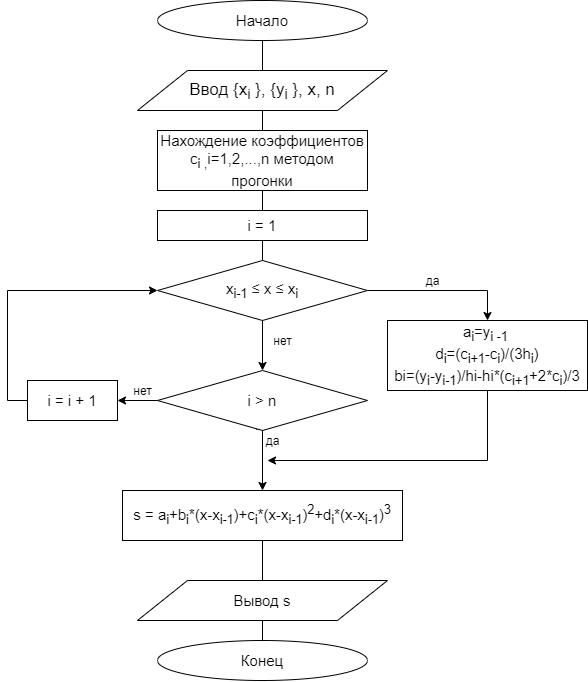
\includegraphics[width = 1\textwidth]{comp-math-lab3.png}
 
\end{figure} 

\newpage

\title{Листинг численного метода}{\begin{center}
    Листинг численного метода
\end{center}} \\
    \begin{verbatim}
        
   
    public void initSplines(double[] x, double[] y) {
         int n = x.length;
        splines = new Spline[n];
        for (int i = 0; i < n; i ++) {
            splines[i] = new Spline();
            splines[i].setX(x[i]);
            splines[i].setA(y[i]);
        }
        splines[0].setC(0d);
        solveByTridiagonalMatrixAlgorithm(x, y, n);
    }

    private void solveByTridiagonalMatrixAlgorithm(double[] x, double[] y, 
    int n) {
        double[] alpha = new double[n - 1];
        double[] beta = new double[n - 1];
        alpha[0] = beta[0] = 0;

        double hi, hi_inc, A = 0, B, C = 0, F = 0, t;

        for (int i = 1; i < n - 1; i ++) {
            hi = x[i] - x[i - 1];
            A = hi;
            hi_inc = x[i + 1] - x[i];
            B = hi_inc;
            C = (hi_inc + hi) * 2;
            F = 6 * ((y[i + 1] - y[i])/hi_inc - (y[i] - y[i - 1])/hi);
            t = (A * alpha[i - 1] + C);

            alpha[i] = -B / t;
            beta[i] = (F - A * beta[i - 1]) / t;
        }
        splines[n - 1].setC((F - A * beta[n - 2])/(C + A * alpha[n - 2]));

        for (int i = n - 2; i > 0; i --)
            splines[i].setC(alpha[i] * splines[i + 1].getC() + beta[i]);

        for (int i = n - 1; i > 0; i --) {
            hi = x[i] - x[i -1];
            splines[i].setD((splines[i].getC() - splines[i - 1].getC()) 
            / hi);
            splines[i].setB((hi * (2 * splines[i].getC() +
            splines[i - 1].getC()) / 6) +
            (y[i] - y[i - 1]) / hi);
        }
    }

    public Function interpolate () {
        return this::getInterpolatedY;
    }

private double getInterpolatedY(double x) {
        Spline spline;
        if (x >= splines[splines.length - 1].getX())
            spline = splines[splines.length - 1];
        else if (x <= splines[0].getX())
            spline = splines[0];
        else {
            int k, left = 0, right = splines.length - 1;
            while (right > left + 1) {
                k = left + (right - left) / 2;
                if (x <= splines[k].getX())
                    right = k;
                else
                    left = k;
            }
            spline = splines[right];
        }
        double dx = x - spline.getX();
        double value = spline.getA() + spline.getB() * dx
                + spline.getC() * dx * dx/2 +
                spline.getD()* dx * dx * dx/6;
        return value;
    }
     \end{verbatim}
\newpage

\title{Примеры}{\begin{center}
    Примеры
\end{center}} \\
\begin{figure}[H]
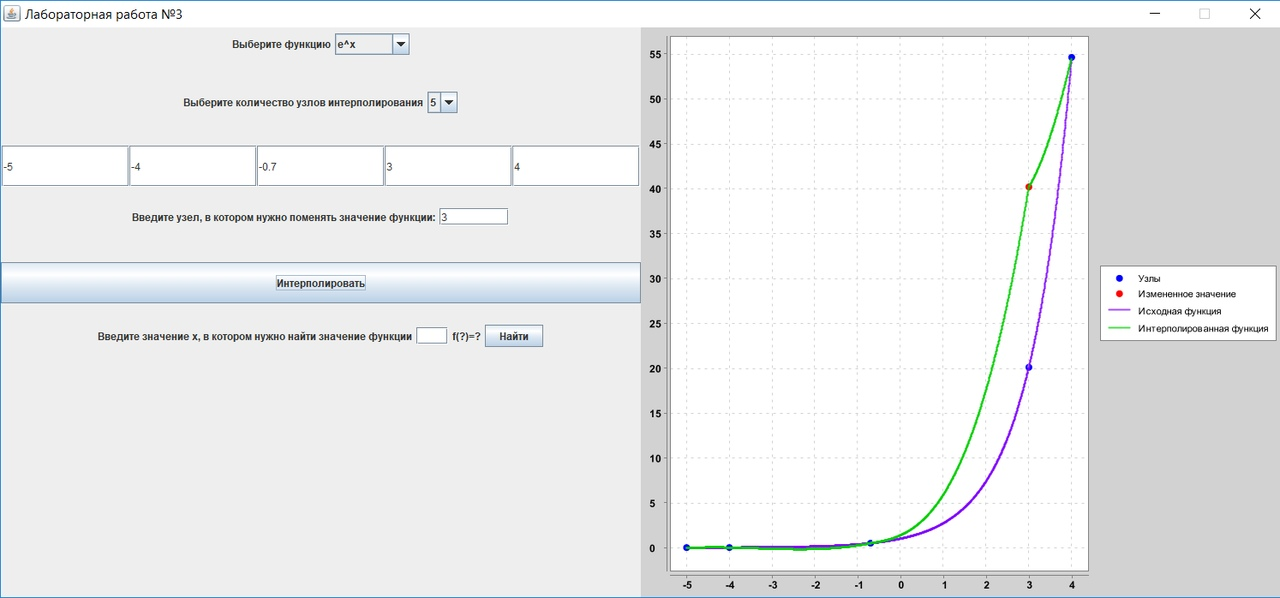
\includegraphics[width = 1\textwidth]{1.jpg}
\end{figure} 

\begin{figure}[H]
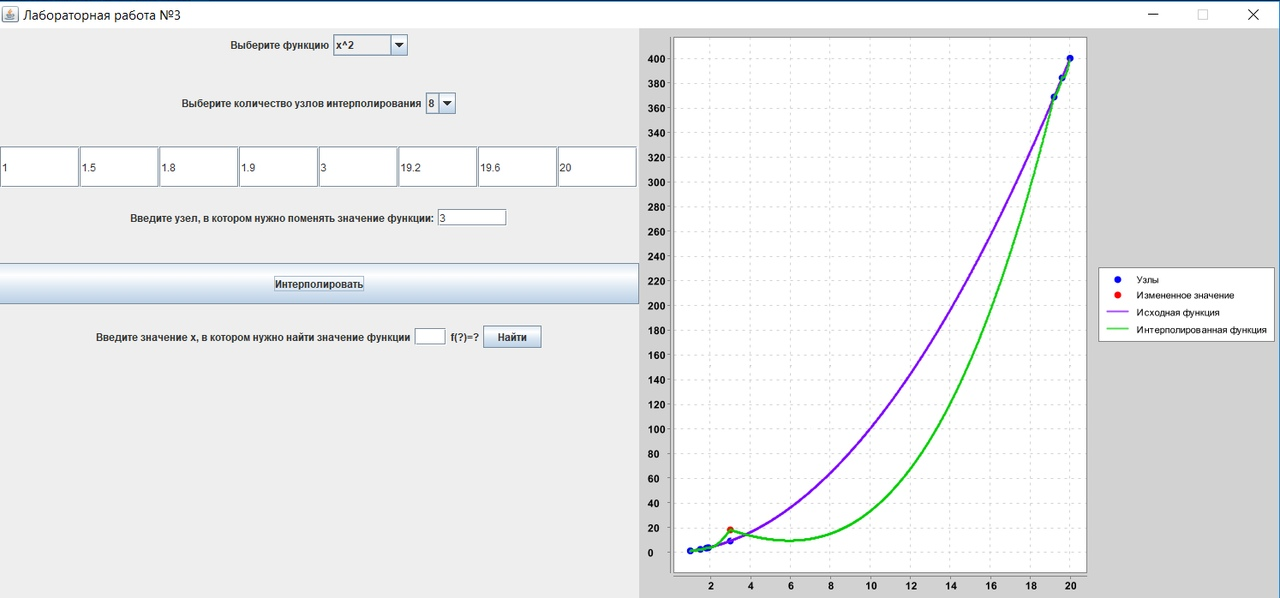
\includegraphics[width = 1\textwidth]{2.jpg}
\end{figure} 

\begin{figure}[H]
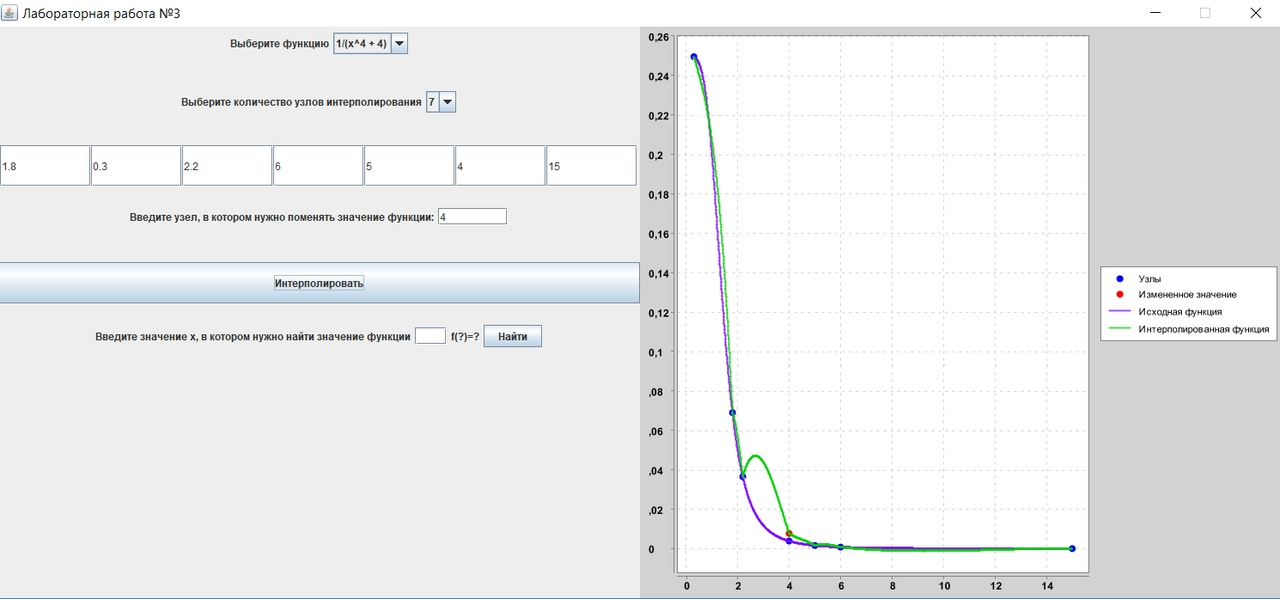
\includegraphics[width = 1\textwidth]{3.jpg}
\end{figure} 



\newpage
   
Вывод: интерполирование кубическими сплайнами - один из способов кусочно-полиноминальной интерполяции, когда весь отрезок разбивают на частичные отрезки и на каждом из частичных отрезков приближенно заменяют исходную функцию многочленом невысокой (в данном случае, третьей степени), в отличие от формул Ньютона и Лагранжа, где отрезок не рабивается. Интерполяцию кубическими сплайнами рационально применять, если f(x) - периодическая или тригонометрическая функция. Что касается других методов интерполяции, а именно формул Ньютона и Лагранжа, то формулу Лагранжа можно применять для таблиц с различными расстояниями между узлами, а формулы Ньютона – только для таблиц с равноотстоящими узлами. Формулы Ньютона имеют следующее преимущество перед формулой Лагранжа: добавление в таблицу узлов интерполяции при использовании формулы Лагранжа ведет к необходимости пересчета каждого коэффициента заново, тогда как при использовании формулы Ньютона достаточно добавить к уже существующему многочлену только одно слагаемое.
Кроме того, по сравнению с этими методами большую точность интерполяции можно получить применением методов сплайн–интерполяции. Что касается сравнения с методом аппроксимации, то следует обратить внимание на разницу в постановке задач аппроксимации и интерполяции: интерполянт должен принадлежать к определенному классу и в точках $x_i (i = 0, 1, ..., n)$ принимать те же значения, что и исходная функция, для аппроксиманта это требование обязательным не является, но должен выполняться критерий наилучшего приближения. В методе наименьших квадратов поле выбора класса аппроксимирующей функции $f(x_i, A, B, C, ...)$ строится сумма вида $Q = \sum\limits_{i=1}^n [f(x_i, A, B, C, ...) - y_i]^2$. Исходными значениями параметров $A, B, C, ...$ полагаются числа,
которые обеспечивают минимум суммы $Q$.